\documentclass[12pt,a4paper]{article}

\usepackage{polski}
\usepackage{graphicx}
\usepackage{caption,subcaption}
\usepackage{makecell}
\usepackage[table]{xcolor}

\usepackage{hyperref}
\hypersetup{
  colorlinks	= true, %Colours links instead of ugly boxes
  urlcolor		= blue, %Colour for external hyperlinks
  linkcolor		= blue, %Colour of internal links
  citecolor		= red 	%Colour of citations
}

\title{Projekt z Podstaw Sztucznej Inteligencji\\
Uczenie maszynowe\\
RB.ML12 Grzyby NN}

\author{
	Rafal Babinski 
\and 
	Roman Moskalenko
}
\date{}


\begin{document}
\maketitle

\section{Treść zadania}

Przewidywanie czy \href{https://archive.ics.uci.edu/ml/datasets/mushroom}{grzyb} jest jadalny przy użyciu własnej implementacji prostej sieci neuronowej.

\section{Interpretacja zadania}

Mamy pełną swobodę w zaimplementowaniu sieci neuronowej. Wykorzystując podany wcześniej zbiór danych, musimy przeanalizować które komponenty sieci i jakie podejście przy jej budowaniu zapewni jak największą efektywność.

\section{Wkład poszczególnych autorów}

Rafal Babinski

\begin{itemize}
	\item	Przygotowanie zbioru danych do przetwarzania
	\item 	Implementacja klasy perceptronu
	\item 	Implementacja K-krotnej walidacji krzyżowej
	\item	Generowanie dokumentacji
\end{itemize}
Roman Moskalenko

\begin{itemize}
	\item 	Implementacja klasy perceptronu
  \item	Generowanie wykresów
  \item	Prowadzenie eksperymentów
\end{itemize}

\section{Decyzje projektowe i przeprowadzone badania}

\subsection{Decyzje wstępne}

\begin{itemize}
	\item 	Wybraliśmy do zaimplementowania prosty lecz efektywny typ sieci neuronowej: perceptron dwuwarstwowy
  \item 	Jako szablon wstępny wybraliśmy sieć neuronową opisaną w tym artykule.
  \item 	Uczenie sieci będzie przeprowadzać się z nadzorem.
  \item 	Przekodowaliśmy podany zbiór danych na kod 1 z n dla zapewnienia działania sieci.
  \item	Arbitralnie wybraliśmy liczbę neuronów w warstwie ukrytej - 2.
  \item 	Arbitralnie wybraliśmy funkcję aktywacji - sigmoid.
  \item 	Inicjalizacja wag każdego neuronu odbywa się losowo.
  \item 	Wartości parametrów bias jest zerowa.
  \item 	Stworzyliśmy zbiór danych kontrolnych, 100 wybranych losowo próbek z podanego zbioru. Na nim będziemy testować efektywność sieci.

\end{itemize}

\pagebreak
\subsection{Badanie wstępne}

\begin{itemize}
	\item 	Uruchomiono po raz pierwszy sieć neuronową.
  \item	Przez 100 iteracji sieć uczyła się na całym zbiorze danych.
  \item 	Przetestowano na losowo wybranych 100 próbkach.
\end{itemize}

\begin{figure}[h]
  \centering
  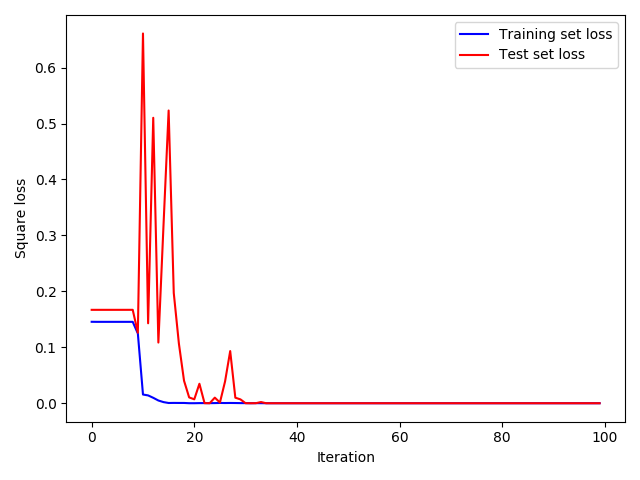
\includegraphics[width=1.0\textwidth]{charts/double_activation/first_chart.png}
  \caption{}
  \label{}
\end{figure}

\begin{itemize}
	\item 	Przez pierwsze 30 iteracji możemy zaobserwować dużą stratę na zbiorze walidacyjnym (czerwona linia).
  \item	Po czym następuje prawie zerowa strata. Mamy podejrzenie, że sieć dopasowała się do danych (przeuczenie sieci).
\end{itemize}

\pagebreak

\subsection{Podział zbioru danych na treningowy i testowy}
Aby zapobiec przeuczeniu sieci dzielimy dane na dwa zbiory: zbiór treningowy --- uczymy na nim sieć, oraz zbiór testowy --- na tym zbiorze sprawdzamy efektywność działania sieci.

\begin{itemize}
  \item   Podział danych na treningowe i testowe w stosunku 1:1.
\end{itemize}

\begin{figure}[h]
  \centering
  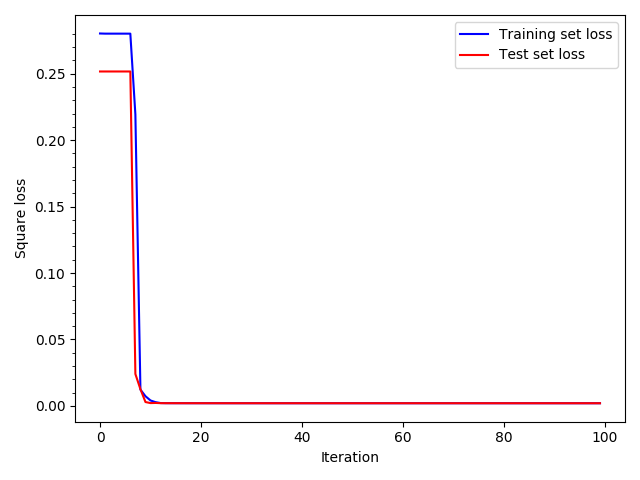
\includegraphics[width=1.0\textwidth]{charts/double_activation/simple_validation_2neurons.png}
  \caption{}
  \label{}
\end{figure}

\begin{itemize}
  \item   Już na 13 iteracji strata na zbiorze testowym osiągnęła 0.002 i utrzymywała się taka w przeciągu pozostałych iteracji.
\end{itemize}

\pagebreak

\subsection{Zależność straty od liczby neuronów i podziału danych}

Badamy jak zmienia się strata na zbiorze testowym w zależności od liczby neuronów i stosunku liczności zbioru treningowego do liczności zbioru testowego.

\begin{itemize}
  \item   Straty po 100 iteracjach uczenia
\end{itemize}

\begin{figure}[h]
  \centering
  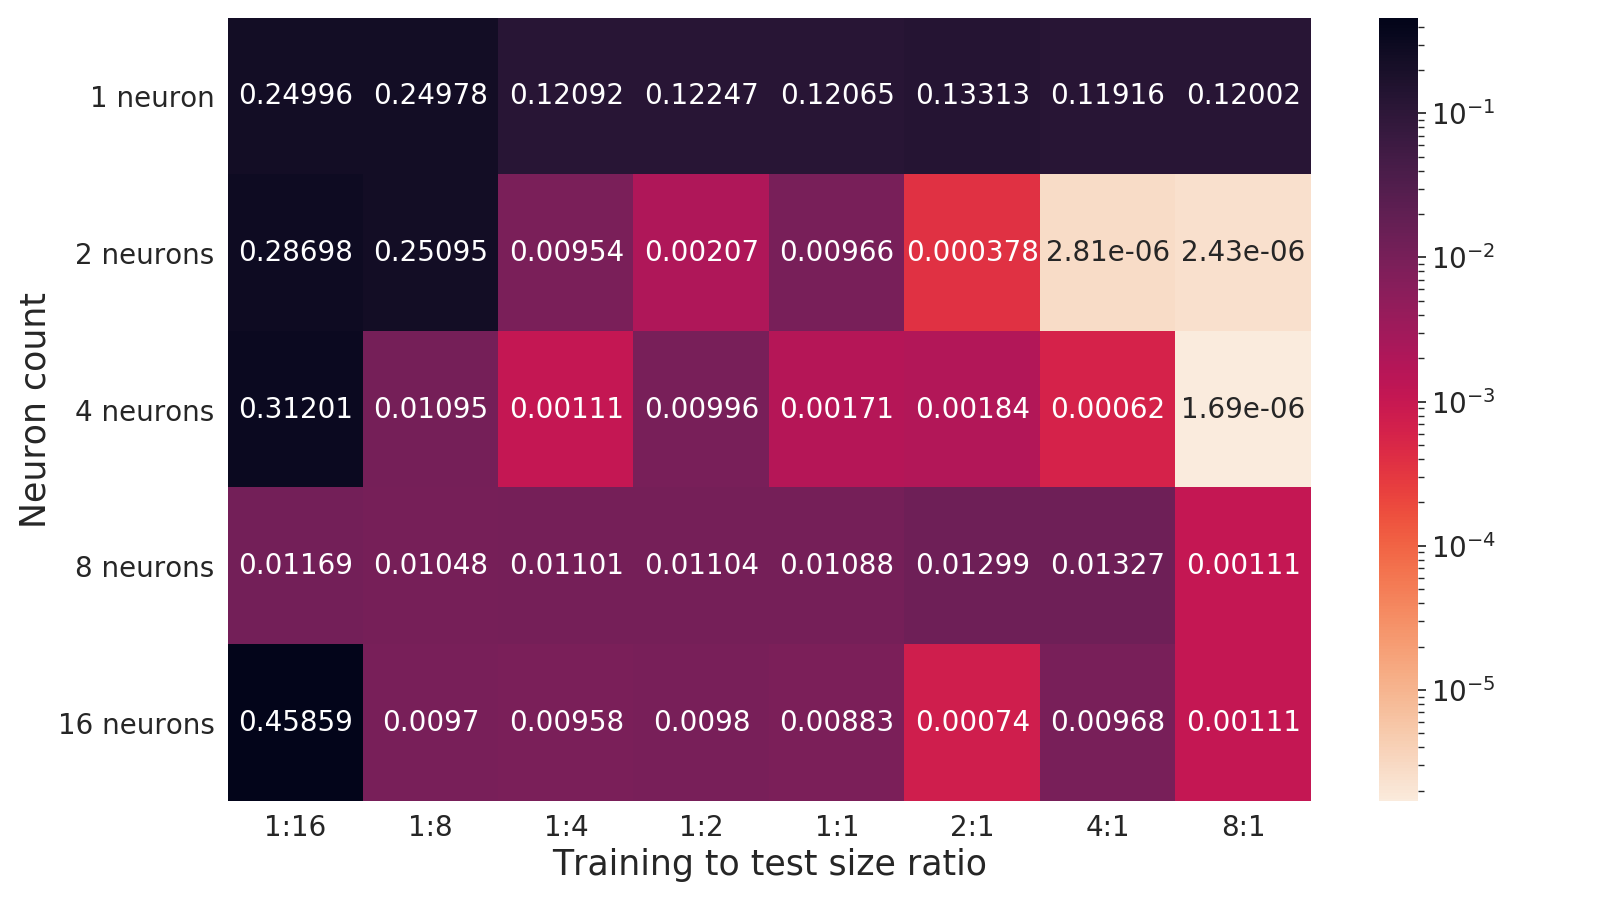
\includegraphics[width=1.0\textwidth]{charts/double_activation/neuron_partition_heattable.png}
  \caption{}
  \label{}
\end{figure}

Wnioski z tabeli:

\begin{itemize}
  \item   Perceptron z 1 neuronem przy żadnym z podziałów nie pokazał dobrych wyników.
  \item   Perceptron z 2 oraz 4 neuronami sprawdził się nieco lepiej niż perceptrony z 8 i 16.
  \item   Perceptron może nauczyć się nawet gdy dane treningowe stanowią połowę lub mniej od całego zbioru lecz wtedy strata jest porównywalnie duża.
  \item   Możliwe, że 100 iteracji to jednak zbyt mało by nauczyć perceptron.
\end{itemize}

\pagebreak

\subsection{Porównanie strat dla większej liczby iteracji dla różnej liczby neuronów}

\begin{itemize}
  \item   Jeszcze dwa razy uruchomiliśmy sieć dla 100 i 400 iteracji dla podziału danych 4:1.
  \item   Wykresy teraz mają skalę logarytmiczną.
\end{itemize}

\begin{figure}[h]
  \centering
\begin{subfigure}{0.5\textwidth}
  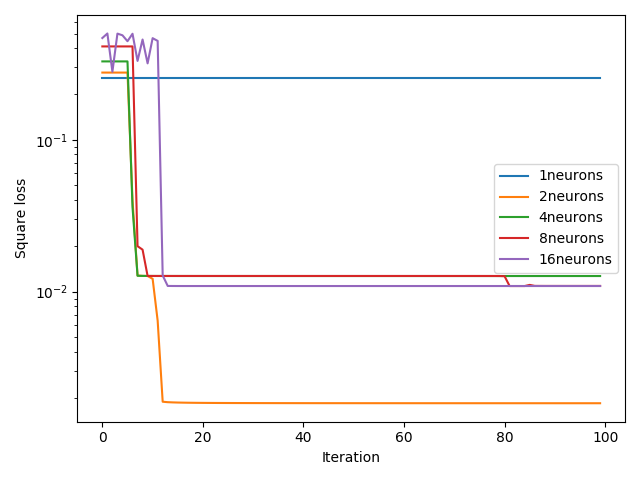
\includegraphics[width=\linewidth]{charts/double_activation/doubleactiv_100iter.png}
  \caption{}
  \label{}
\end{subfigure}\hfil
\begin{subfigure}{0.5\textwidth}
  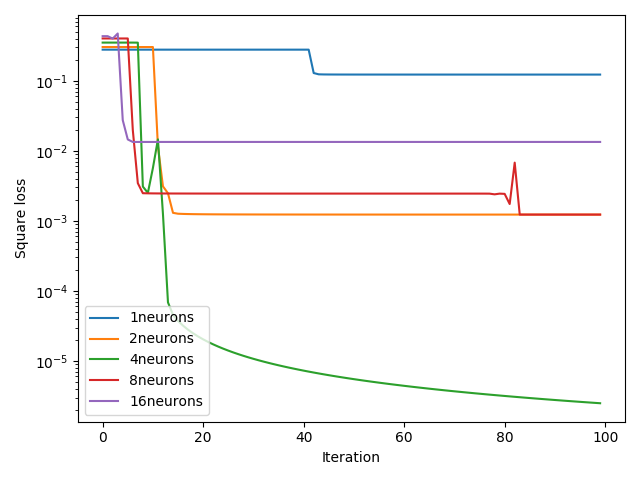
\includegraphics[width=\linewidth]{charts/double_activation/doubleactiv_100iter2.png}
  \caption{}
  \label{}
\end{subfigure}

\medskip
\begin{subfigure}{0.5\textwidth}
  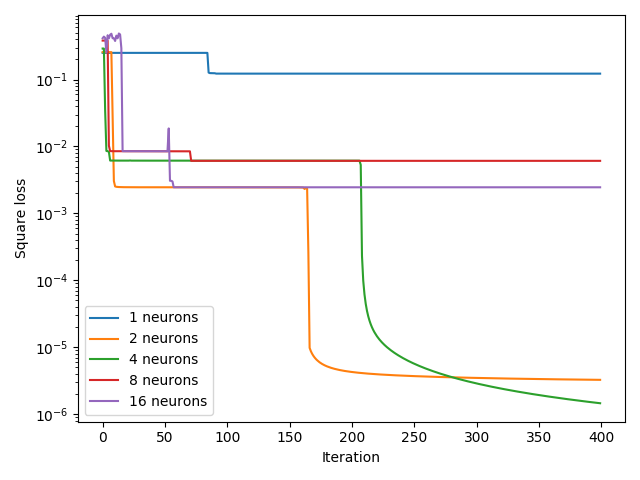
\includegraphics[width=\linewidth]{charts/double_activation/doubleactiv_400iter.png}
  \caption{}
  \label{}
\end{subfigure}\hfil
\begin{subfigure}{0.5\textwidth}
  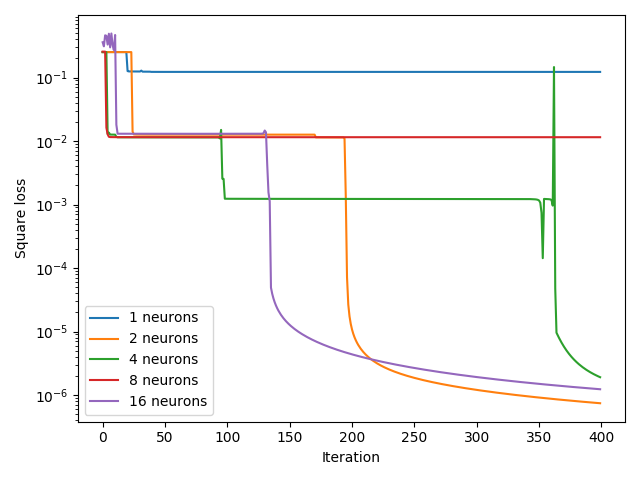
\includegraphics[width=\linewidth]{charts/double_activation/doubleactiv_400iter2.png}
  \caption{}
  \label{}
\end{subfigure}

\end{figure}

Widać, że liczba iteracji ma duże znaczenie. Większość wariacji perceptronu zmniejsza stratę dopiero po 100 iteracjach. Jednak ciężko przewidzieć w którym momencie nastąpi zmniejszenie straty i czy w ogóle nastąpi.

\pagebreak

\subsection{Modyfikacja perceptronu}

Ponieważ nasz perceptron jest implementacją bazowaną na przykładzie z artykułu powyżej, może zawierać wady, z powodu możliwych uproszczeń przyjętych w artykule.

Z tego powodu następujące zmiany powinny zbliżyć naszą implementacje do modelu przedstawionego na wykładzie:

\begin{itemize}
  \item   Neuron warstwy wyjściowej jest liniowy (nie obliczamy funkcji aktywacji dla niego).
  \item   Odpowiednie zmiany propagacji wstecznej.
\end{itemize}

\begin{itemize}
  \item   Straty po 100 iteracjach uczenia
\end{itemize}

\begin{figure}[h]
  \centering
  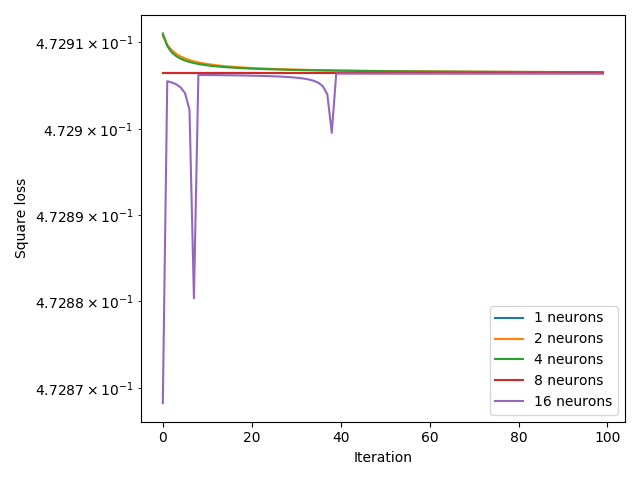
\includegraphics[width=1.0\textwidth]{charts/no_output_activation/noactiv100iter_lr1.png}
  \caption{}
  \label{}
\end{figure}

\begin{itemize}
  \item   Strata prawię się nie zmienia dla wszystkich wariacji perceprtonu i wynosi w przybliżeniu 0.4729.
  \item   W czasie działania programu dostaliśmy warning o nadmiarze zauważonym przy obliczaniu funkji aktywacji: 
RuntimeWarning: overflow encountered in exp: return 1 / (1 + np.exp(-x))
\end{itemize}

Okazuje się, że po usunięciu funkcji aktywacji (i jej pochodnej w propagacji wstecznej) pochodna po wagach staje się zbyt duża, co skutkuje tym, że wartości bezwzględne wag stają się zbyt duże i powodują powstanie nadmiaru przy obliczaniu funkcji aktywacji.

Chcemy mieć kontrolę nad tym jak szybko zmieniają się wagi. Wprowadzamy tzw współczynnik uczenia. Teraz pochodne straty zanim dodać do wag przemnażamy przez ten parametr. Dla początku przyjęliśmy współczynnik uczenia równy 0.1.

\begin{figure}[h]
  \centering
\begin{subfigure}{0.5\textwidth}
  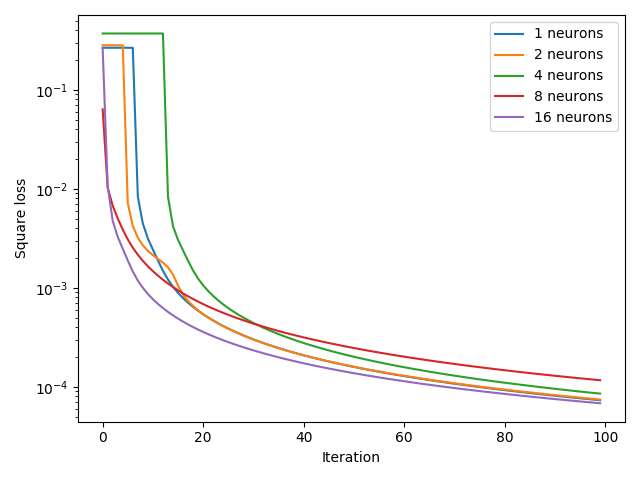
\includegraphics[width=\linewidth]{charts/no_output_activation/noactiv100iter_lr01_randw.png}
  \caption{}
  \label{}
\end{subfigure}\hfil
\begin{subfigure}{0.5\textwidth}
  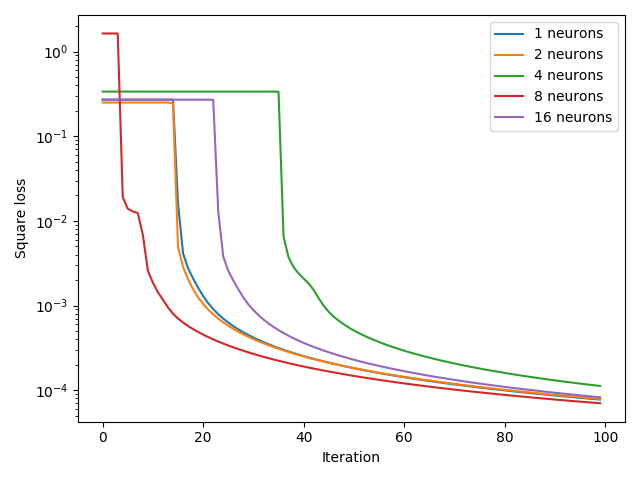
\includegraphics[width=\linewidth]{charts/no_output_activation/noactiv100iter_lr01_randw2.png}
  \caption{}
  \label{}
\end{subfigure}

\medskip
\begin{subfigure}{0.5\textwidth}
  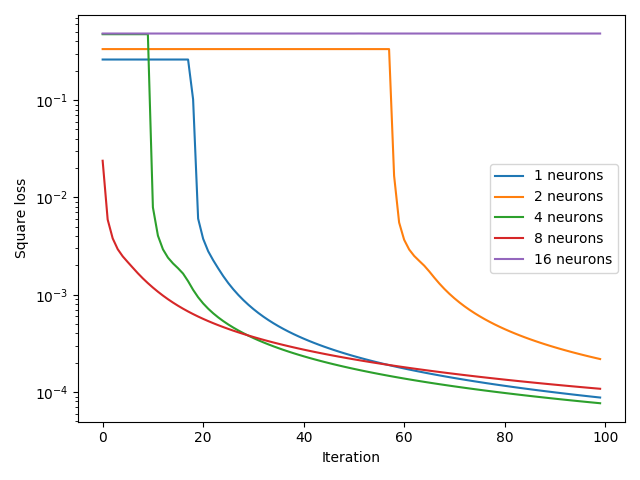
\includegraphics[width=\linewidth]{charts/no_output_activation/noactiv100iter_lr01_randw3.png}
  \caption{}
  \label{}
\end{subfigure}

\end{figure}

\begin{itemize}
  \item   obserwujemy wyraźne poprawienie sprawności
  \item   zauważalny jest wpływ losowości początkowych wag
\end{itemize}

\pagebreak

\subsection{Inicjowanie wag}

Wolimy zmniejszyć do minimum negatywny wpływ losowości wag.

\begin{itemize}
  \item   Inicjujemy wagi neuronu wyjściowego zerami zamiast robić to losowo.
  \item   Wagi neuronów ukrytych losujemy z rozkładu jednostajnego z przedziału \((-\frac{1}{\sqrt{n}}, \frac{1}{\sqrt{n}})\), gdzie n - wymiar wymiar wejścia neuronu.
\end{itemize}

\begin{figure}[h]
  \centering
\begin{subfigure}{0.5\textwidth}
  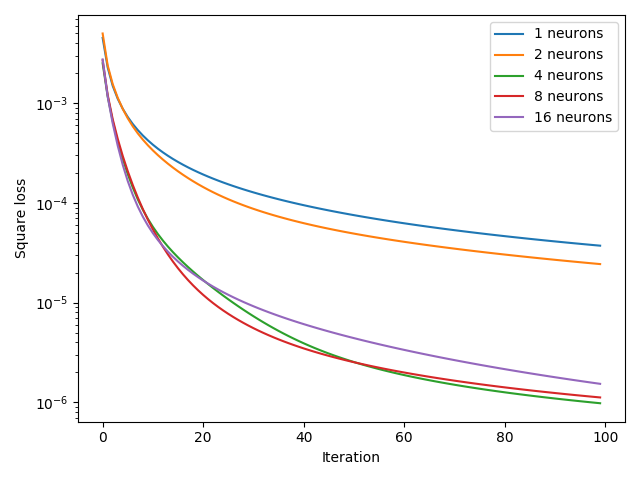
\includegraphics[width=\linewidth]{charts/no_output_activation/noactiv400iter_lr01_custw.png}
  \caption{}
  \label{}
\end{subfigure}\hfil
\begin{subfigure}{0.5\textwidth}
  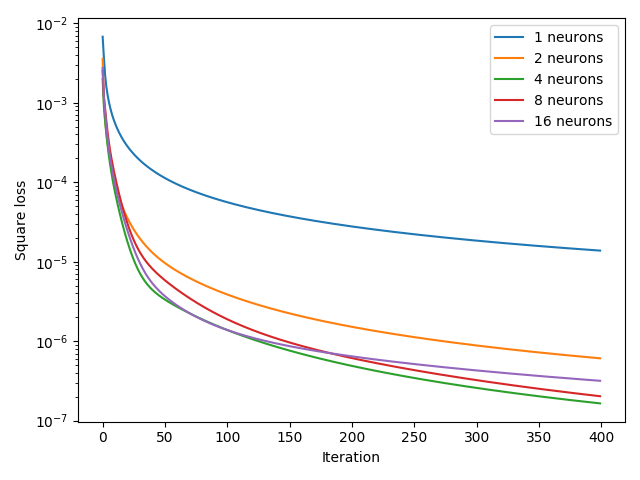
\includegraphics[width=\linewidth]{charts/no_output_activation/noactiv400iter_lr01_custw2.png}
  \caption{}
  \label{}
\end{subfigure}

\end{figure}

\begin{itemize}
  \item   Obserwujemy bardzo dobry rezultat.
  \item   Perceptron natychmiast zaczyna poprawiać stratę dla wszystkich badanych wariacji.
  \item   Perceptron z 1 i 2 neuronami uczy się wolno w porównaniu z innymi.
  \item   Perceptron z 16 neuronami już nie poprawia wyniku w porównaniu z 4 czy 8 neuronami.
\end{itemize}

\pagebreak

\subsection{Zależność sprawności perceptronu od współczynnika uczenia}

Porównamy jak zachowuje się strata dla perceptronu z 4 neuronami dla różnych współczynników uczenia.

\begin{figure}[h]
  \centering
  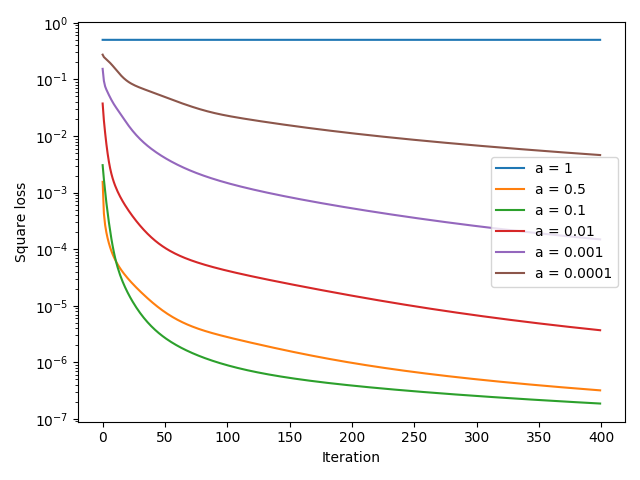
\includegraphics[width=\linewidth]{charts/learning_rates/4neurons.png}
  \caption{}
  \label{}
\end{figure}

\begin{itemize}
  \item   Zbyt mały współczynnik uczenia powoduje, że sieć uczy się zbyt wolno.
  \item   Zbyt duży współczynnik skutkuje zbyt częstymi błędami sieci, a więc dużą stratą.
\end{itemize}

\pagebreak

Porównamy teraz straty dla wspóczynników uczenia 0.07, 0.1 oraz 0.3 dla perceptronów z 4 i 8 neuronami.

\begin{figure}[h]
  \centering
\begin{subfigure}{0.5\textwidth}
  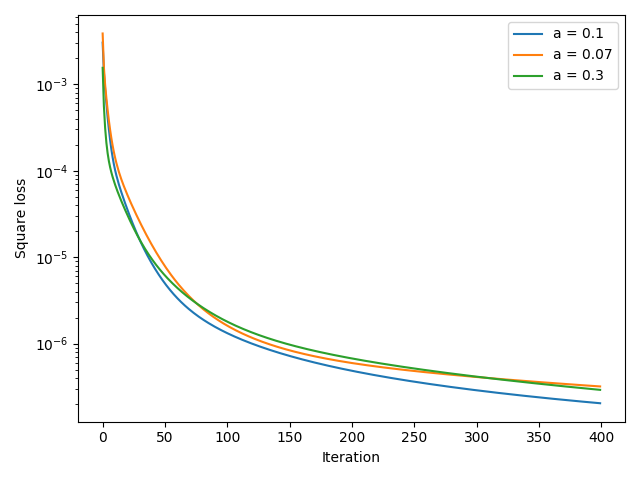
\includegraphics[width=\linewidth]{charts/learning_rates/4neurons2.png}
  \caption{4 neurony}
  \label{}
\end{subfigure}\hfil
\begin{subfigure}{0.5\textwidth}
  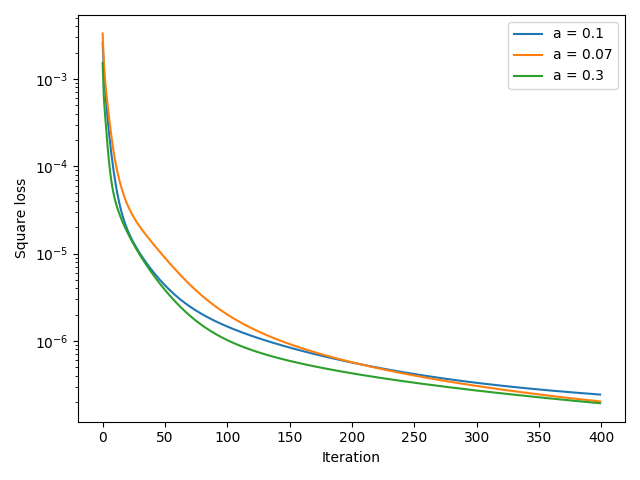
\includegraphics[width=\linewidth]{charts/learning_rates/8neurons.png}
  \caption{8 neuronów}
  \label{}
\end{subfigure}
\caption{Porównanie współczynników uczenia 0.07, 0.1 oraz 0.3}
\label{}
\end{figure}

\begin{itemize}
  \item   współczynniki jakości pokazują porównywalny rezultat
  \item   postanowiliśmy w dalszych eksperymentach używać wartości 0.1
\end{itemize}

\subsection{K-krotna walidacja krzyżowa}

Dla ulepszenia jakości uczenia i oceniania sieci wprowadzamy metodę k-krotnej walidacji krzyżowej. Rysunek poniżej ilustruje w jaki sposób dzielone są dane wejściowe.

\begin{figure}[h]
  \centering
  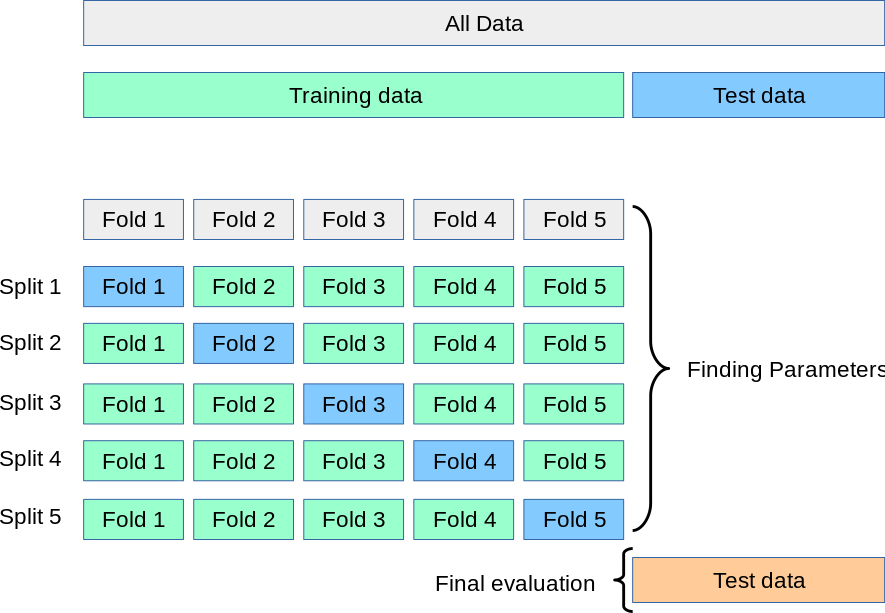
\includegraphics[width=0.62\textwidth]{charts/grid_search_cross_validation.png}
  \caption{}
  \label{}
\end{figure}

Początkowy zbiór dzielony jest na:

\begin{itemize}
  \item   Zbiór walidacyjny, na którym sieć się nie uczy, sprawdzamy na nim poprawność sprawność sieci.
  \item   Zbiór przetwarzany przez sieć metodą k-krotnej walidacji.
\end{itemize}

Tabela poniżej pokazuje liczbę poprawnie przewidzianych odpowiedzi i odpowiednie parametry sieci.
 
\begin{table}[h]
\centering
\resizebox{\textwidth}{!}
{\rowcolors{2}{blue!80!yellow!10}{blue!70!yellow!0}
\begin{tabular}{ |c|c|c|c|c|c| }
  \hline
  \textbf{\thead{Liczba \\iteracji \\uczenia}} & \textbf{\thead{Liczba \\neuronów}} & \textbf{\thead{Współczynnik \\uczenia}} & \textbf{\thead{Stosunek \\zbiorów}} & \textbf{\thead{Poprawne \\odpowiedzi}} & \textbf{Strata} \\
  \hline
  100 & 4 & 0.1 & 16:4:5 & 1624/1624 & 2.168e-07 \\
  \hline
  50 &	2 &	0.1 &	16:4:5 & 1624/1624 & 1.382e-06 \\
  \hline
  10 &	1 &	0.1 &	8:2:5 &	2708/2708 &	0.00012544 \\
  \hline
  10 &	1 &	0.1 &	2:1:3 &	4062/4062 &	0.00030634 \\
  \hline
  1 &	1 &	0.1 &	1:1:2 &	4055/4062 &	0.00486307 \\
  \hline
  1 &	1 &	0.001 &	1:1:2 &	3662/4062 &	0.09289285 \\
  \hline
  
\end{tabular}}
\end{table}

Widać, że nawet bardzo słabo nauczona sieć na jednym neuronie potrafi poprawnie przewidywać wszystkie próbki ze zbioru walidacyjnego, co mówi o tym, że zależność tego czy grzyb jest jadalny czy nie od jego parametrów jest bardzo prosta.

\subsection{Porównanie perceptronu z funkcją aktywacji na neuronach warstwy wyjściowej i bez niej}

Konfiguracja:

\begin{itemize}
  \item   4 neurony
  \item   współczynnik uczenia 0.1
  \item   stosunek danych walidacyjnych do pozostałych 1:1
  \item   stosunek danych treningowych do testowych 2:1
  \item   liczba iteracji uczenia na każdym k-krotnym podziale 100
  \item   liczba iteracji uczenia po k-krotnej walidacji 100
  \item   ziarno losowości 1
\end{itemize}

\begin{table}[h]
\centering
\begin{tabular}{ |c|c|c| }
  \hline
  & \textbf{Z funkcją aktywacji} & \textbf{Bez funkcji aktywacji} \\ [0.5ex] 
  \hline
  \textbf{\thead{Strata \\uśredniona testowa}} & 4.84142896e-06 & 1.69846478e-06\\
  \hline
  \textbf{\thead{Strata \\na zbiorze walidacyjnym}} & 5.49349119e-06 & 4.38600909e-07 \\
  \hline
  \textbf{\thead{Poprawne \\odpowiedzi}} & 100.0\% & 100.0\% \\
  \hline  
\end{tabular}
\end{table}

\begin{figure}[h]
  \centering
\begin{subfigure}{0.5\textwidth}
  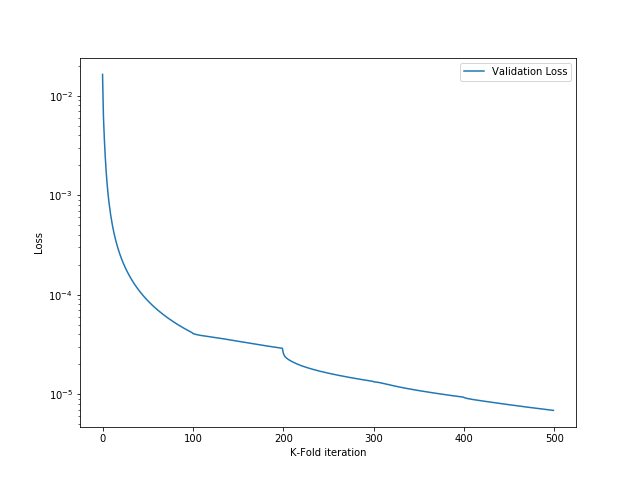
\includegraphics[width=\linewidth]{charts/activ_vs_noactiv/activ.png}
  \caption{Z funkcją aktywacji}
  \label{}
\end{subfigure}\hfil
\begin{subfigure}{0.5\textwidth}
  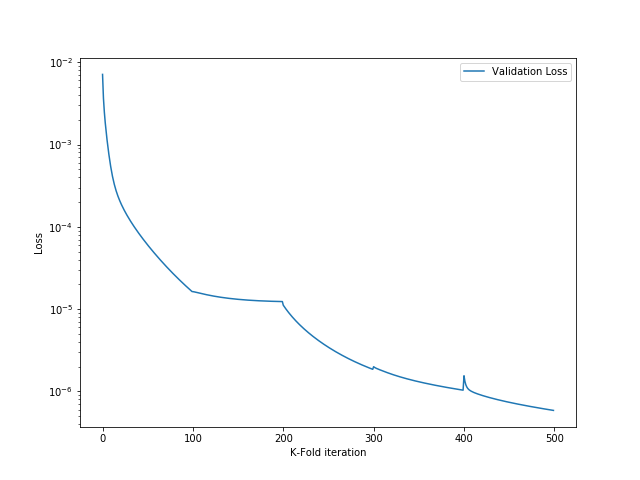
\includegraphics[width=\linewidth]{charts/activ_vs_noactiv/noactiv.png}
  \caption{Bez funkcji aktywacji}
  \label{}
\end{subfigure}
\caption{Wykres zależności straty na zbiorze walidacyjnym od iteracji}
\label{}
\end{figure}

Przeprowadzimy jeszcze raz takie same testy przy gorszych warunkach:

\begin{itemize}
  \item   1 neuron
  \item   współczynnik uczenia 0.001
  \item   stosunek danych walidacyjnych do pozostałych 1:1
  \item   stosunek danych treningowych do testowych 1:1
  \item   liczba iteracji uczenia na każdym k-krotnym podziale 100
  \item   liczba iteracji uczenia po k-krotnej walidacji 100  
  \item   ziarno losowości 1  
\end{itemize}

\pagebreak

\begin{table}[h]
\centering
\begin{tabular}{ |c|c|c| }
  \hline
  & \textbf{Z funkcją aktywacji} & \textbf{Bez funkcji aktywacji} \\ [0.5ex] 
  \hline
  \textbf{\thead{Strata \\uśredniona testowa}} & 0.1414469073940681 & 0.010690605358111328 \\
  \hline
  \textbf{\thead{Strata \\na zbiorze walidacyjnym}} & 0.12473975 & 0.00486256 \\
  \hline
  \textbf{\thead{Poprawne \\odpowiedzi}} & 53.18\% & 99.88\% \\
  \hline  
\end{tabular}
\end{table}

\begin{figure}[h]
  \centering
\begin{subfigure}{0.5\textwidth}
  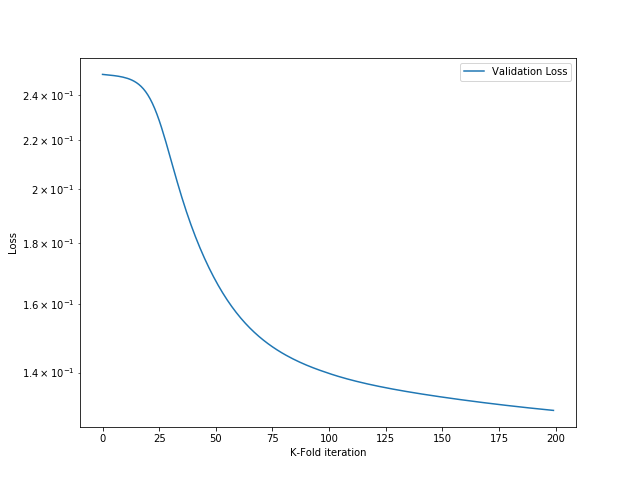
\includegraphics[width=\linewidth]{charts/activ_vs_noactiv/activ_extr.png}
  \caption{Z funkcją aktywacji}
  \label{}
\end{subfigure}\hfil
\begin{subfigure}{0.5\textwidth}
  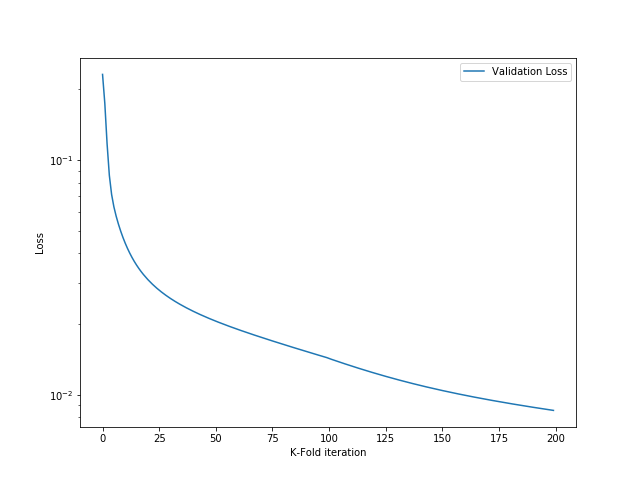
\includegraphics[width=\linewidth]{charts/activ_vs_noactiv/noactiv_extr.png}
  \caption{Bez funkcji aktywacji}
  \label{}
\end{subfigure}
\caption{Wykres zależności straty na zbiorze walidacyjnym od iteracji}
\label{}
\end{figure}

Perceptron bez funkcji aktywacji na neuronie wyjściowym na ogół wykazuje mniejszą stratę i pokazuje nieco lepsze wyniki niż w przypadku z funkcją aktywacji.

\section{Podsumowanie badań}

Pod koniec badań większość wariacji perceptronu pokazywała dobre wyniki i często miała 100\% poprawnych odpowiedzi na zbiorze walidacyjnym.

Natomiast najmniejszą możliwą stratę wykazuję dana modyfikacja perceptronu:

\begin{itemize}
  \item   4-8 neuronów
  \item   Współczynnik uczenia 0.1
  \item   Sygmoidalna funkcja aktywacji na neuronach warstwy ukrytej
  \item   Liniowy neuron wyjściowy (bez funkcji aktywacji)
  \item   Losowe inicjowanie wag neuronów warstwy ukrytej z rozkładu jednostajnego \(U ~ (-\frac{1}{\sqrt{n}}, \frac{1}{\sqrt{n}})\)
  \item   Inicjowanie wag neuronu wyjściowego zerami
  \item   Współczynnik k równy 4 bądź 5 dla K-krotnej walidacji krzyżowej
\end{itemize}

\section{Listę wykorzystanych narzędzi i bibliotek}

Język programowania

\begin{itemize}
	\item   Python 3
\end{itemize}

Wykorzystane biblioteki

\begin{itemize}
	\item   \href{https://numpy.org/}{numpy}
	\item   \href{https://pandas.pydata.org/}{pandas}
	\item   \href{https://seaborn.pydata.org/}{seaborn}
\end{itemize}

Wykorzystane materiały

\begin{itemize}
	\item   \url{https://scikit-learn.org/stable/modules/cross_validation.html}
\end{itemize}

\end{document}